\begin{python0}
from solutions import *; clear()
\end{python0}
\sectionthree{More examples}

\begin{ex}
Can you create a reference that refers to a reference?

\begin{consolethree}[escapeinside=||]
double i = 3.14;
double & j = i;
double & k = j; // k references j which references i

i = 2.718;
std::cout << i << ' ' << j << ' ' << k << std::endl;

j = 1.414;
std::cout << i << ' ' << j << ' ' << j << std::endl;

k = 0.693;
std::cout << i << ' ' << j << ' ' << j << std::endl;
\end{consolethree}
\end{ex}
\sidenote
{
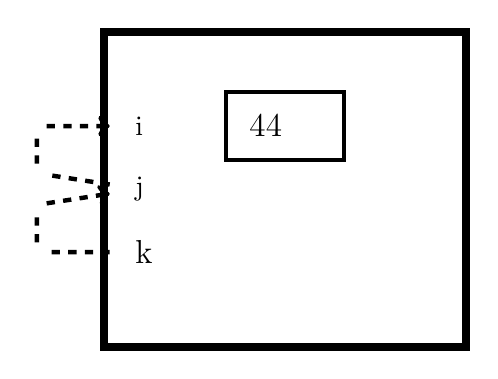
\begin{tikzpicture}
    \node[draw,text width=4cm,minimum height=4cm,minimum width=2cm, line width=0.1cm, inner sep=0.3cm] (a) at (-4, 2) {};
    \node[xshift=-8mm, yshift=8mm] (ji_arr) at (a.west) {};
    \node[xshift=-8mm, yshift=-8mm] (k_arr) at (a.west) {};
    \node[xshift=-8mm, yshift=2mm] (j_arr) at (a.west) {};
    \node[xshift=-8mm, yshift=-2mm] (kj_arr) at (a.west) {};

    \node[text width=1mm,minimum height=1mm,minimum width=1mm, line width=0.05cm, inner sep=0.3cm, xshift=5mm, yshift=8mm] (ival) at (a.west) {\normalsize{i}};
    \node[draw, text width=9mm,minimum height=1mm,minimum width=5mm, line width=0.05cm, inner sep=0.3cm, yshift=8mm] (ivalbox) at (a.center) {\large{44}};
    \node[text width=1mm,minimum height=1mm,minimum width=1mm, line width=0.05cm, inner sep=0.3cm, xshift=5mm] (jval) at (a.west) {\normalsize{j}};

    \node[text width=1mm,minimum height=1mm,minimum width=1mm, line width=0.05cm, inner sep=0.3cm, xshift=5mm, yshift=-8mm] (kval) at (a.west) {\large{k}};

   \draw [dashed, ultra thick, ->] (kval)[xshift=1mm] -- (k_arr) -- (kj_arr) -- (jval)[xshift=1mm];
   \draw [dashed, ultra thick, ->] (jval)[xshift=1mm] -- (j_arr) -- (ji_arr) -- (ival)[xshift=1mm];

\end{tikzpicture}
}
Here's the relevant rule: \EMPHASIZE{A reference can refer to another reference}. In other words, a reference variable can reference a variable or it can reference another reference variable.

\begin{ex}
What is the output?

\begin{consolethree}[escapeinside=||]
void f(int & a, double c)
{
    a = a + int(c);
    c = 1.0;
}

void g(int & b, double & c)
{
    b *= 2 + int(c);
    c = 0.0;
    f(b, c);
}

int main()
{
    int x = 42;
    double y = 3.14;
    g(x, y);
    std::cout << x << ' ' << y << std::endl;
    return 0;
}
\end{consolethree}

(Suggestion: Drawing a memory model might help.)
\end{ex}

Here's another rule: \EMPHASIZE{References must be initialized. Once you declare a reference, it must immediately refer to the memory of another variable}. Try this:

\begin{consolethree}[escapeinside=||]
int i = 5;
int & j; // create a reference variable ...
j = i;   // ... and *then* make the reference
\end{consolethree}

\begin{ex}
Does this work?

\begin{consolethree}[escapeinside=||]
int i = 5;
int & j = i + 1;
\end{consolethree}

Or this?

\begin{consolethree}[escapeinside=||]
int i = 5;
int k = 6;
int & j = i + k;
\end{consolethree}

Why?
\end{ex}

Yet another rule: \EMPHASIZE{Variable references must be initialized to variables or another reference (not an expression)} (This one is kind of obvious.) Here's an example:

\begin{ex}
Of course you know that you can do this:

\begin{consolethree}[escapeinside=||]
double x = 3.14;
int y = x;
\end{consolethree}

What about this:

\begin{consolethree}[escapeinside=||]
double x = 3.14;
int & y = x;
\end{consolethree}
\end{ex}

Rules, rules, rules ... \EMPHASIZE{The type of a reference must match the type it's referring to}.

\begin{ex}
What is the output? (Or find the errors).

\begin{consolethree}[escapeinside=||]
void swap(int & b, int & c)
{
    int t = b;
    b = c;
    c = t;
}

int main()
{
    int x = 42;
    double y = 1.234;
    swap(x, y);
    std::cout << x << ' ' << y << std::endl;
    return 0;
}
\end{consolethree}
\end{ex}

\begin{ex}
What is the output? (Or is there an error?)

\begin{consolethree}[escapeinside=||]
void g(double & b, double & c)
{
    b *= 2 + int(c);
    c = 0.0;
}

int main()
{
    int x = 42;
    double y = 3.14;
    g(x, y);
    std::cout << x << ' ' << y << std::endl;
    return 0;
}
\end{consolethree}

(Suggestion: Drawing a memory model might help.)
\end{ex}

\begin{ex}
You now know this works:

\begin{consolethree}[escapeinside=||]
int i = 0;
int & a = i;
\end{consolethree}

What about the following?

\begin{consolethree}[escapeinside=||]
int i = 0;
const int & a = i;
\end{consolethree}

\begin{consolethree}[escapeinside=||]
const int i = 0;
const int & a = i;
\end{consolethree}

\begin{consolethree}[escapeinside=||]
const int i = 0;
int & a = i;
\end{consolethree}

Try all of them. Give a reason for those that does not work. For those that work, can you change the value of \texttt{i} using \texttt{i}?

\verb!i = 42;!

Can you change the value of \texttt{i} using \texttt{a}?

\verb!a = 42;!

Why?
\end{ex}

\begin{ex}
What is the output? (Or find all the errors).

\begin{consolethree}[escapeinside=||]
void g(const int & b, const double & c)
{
    b *= 2 + c;
    c = 0.0;
    f(b, c);
}

int main()
{
    const int x = 42;
    double y = 3.14;
    g(x, y);
    std::cout << x << ' ' << y << std::endl;
    return 0;
}
\end{consolethree}
\end{ex}

\begin{ex}
What is the output? (Or find all the errors).

\begin{consolethree}[escapeinside=||]
void g(int & b, const double & c)
{
    b *= 2 + c;
    c = 0.0;
    f(b, c);
}

int main()
{
    const int x = 42;
    double y = 3.14;
    g(x, y);
    std::cout << x << ' ' << y << std::endl;
    return 0;
}
\end{consolethree}
\end{ex}

As mentioned before, a variable reference must reference a variable (or another reference). One exception is that \EMPHASIZE{a constant reference can refer to a constant}. Try this:

\verb!const int & i = 5;!

On the other hand the following won't work since you
already know that a reference must refer to a variable:

\verb!int & i = 5;!

A \EMPHASIZE{constant reference} is a reference that refers to a value and
treat that value as a constant.

\begin{consolethree}[escapeinside=||]
int x = 42;
const int & y = x; // y is a const ref to x

const int a = 0;
const int & b = a; // b is a const ref to a
\end{consolethree}

It's very important to remember that if \texttt{x} is a non-constant variable and \texttt{y} is a constant reference to \texttt{x}, then you cannot change the value of \texttt{x} using \texttt{y} -- because \texttt{y} views the value of \texttt{x} as though it's constant. However \texttt{x} can still change it's value:

\begin{consolethree}[escapeinside=||]
int x = 42;
const int & y = x;
std::cout << x << ' ' << y << '\n'

x = 0; // changing x ... OK
std::cout << x << ' ' << y << '\n'

y = -1; // changing x using y ... BAD!!!
\end{consolethree}

\begin{ex}
What is the output? (Or find the error)

\begin{consolethree}[escapeinside=||]
#include <iostream>

int f(int x[], int & len)
{
    int p = 1;
    for (int i = 0; i < len; i++)
    {
        p *= x[i];
    }
    return p;
}

int main()
{
    int a[] = {1, 2, 3};
    std::cout << f(a, 3) << std::endl;
    return 0;
}
\end{consolethree}
\end{ex}

\begin{ex}
After declaring a reference can the reference change the variable it's referring to? Does = work?

\begin{consolethree}[escapeinside=||]
int x = 1;
int y = 2;
int & z = x; // make z refer to x
z = 0;
std::cout << x << ' ' << y << ' ' << z << std::endl;

z = y; // make z refer to y ... can we?
z = -1;
std::cout << x << ' ' << y << ' ' << z << std::endl;
\end{consolethree}
\end{ex}

Here the rule: \EMPHASIZE{a reference variable cannot refer to another variable after it's initialization.}


